\newcommand{\myfontsize}{11pt}


\documentclass[\myfontsize, letterpaper]{article}

\usepackage[margin=1.0in]{geometry}
\usepackage{color}
\usepackage{times}
\usepackage{amssymb}
\usepackage[labelfont=bf, font=scriptsize]{caption}
\usepackage{graphicx}
\usepackage{cite}
\usepackage{multicol}
\usepackage{amsmath}
\usepackage{setspace}
\usepackage{subfigure}


\usepackage{enumerate}

% TOGGLE MULTIPLE COLUMNS
\usepackage{etoolbox}
\newtoggle{cols}
\toggletrue{cols}
\togglefalse{cols}


\iftoggle{cols}{
    \newcommand{\myfigure}{figure*}
    \newcommand{\mytable}{table*}
}{
    \newcommand{\myfigure}{figure}
    \newcommand{\mytable}{table}
}



% linking
\usepackage{hyperref}

%TODO:
%apostrophes aren't showing up
%fix figures (use PS versions for high-res)
%fix paragraph indentation

% Add paragraph numbering, allows for numbering up to 5 levels deep.
% http://pleasemakeanote.blogspot.com/2010/06/how-to-activate-subsubsubsection-in.html
\setcounter{secnumdepth}{5}

% get rid of badness warnings in bibliography
% http://tex.stackexchange.com/questions/10924/underfull-hbox-in-bibliography
\usepackage{etoolbox}
\apptocmd{\sloppy}{\hbadness 10000\relax}{}{}

% adds line breaks after paragraph section headings
% http://tex.stackexchange.com/questions/32160/new-line-after-paragraph
\newcommand{\myparagraph}[1]{\paragraph{#1}\mbox{}\\[\myfontsize]}
\newcommand{\projectname}{VM2Docker}

\author{
    Eric Lubin\\
    \href{mailto:eblubin@mit.edu}{eblubin@mit.edu}
\\\\
    Thesis Advisor: \\
Martin Rinard, Professor MIT\\
    \href{mailto:rinard@csail.mit.edu}{rinard@lcs.mit.edu}
\\\\
Mentor:\\
Jim Yang, VMware \\
\href{mailto:jimyang@vmware.com}{jimyang@vmware.com}\\
}


\title{\projectname: Automating the Conversion from Virtual Machine to Docker Container \\[1\baselineskip] \Large{M.Eng Thesis Proposal}}

\begin{document}
\maketitle
\iftoggle{cols} {
    \begin{multicols}{2}
}
\doublespacing
\section{Introduction}
Historically, virtual machines have owned a staggering majority of the enterprise marketplaces. Recently, a relatively new framework called Docker hopes to redefine the industry. Making use of many extensions to the Linux kernel, Docker containers are a lightweight alternative to virtual machines that aim to streamline the developer workflow by creating shippable build environments without the bulk and performance degradation of running within a virtual machine.

Unlike virtual machines, containers share the kernel with the host and other containers running on that same host. For this reason, Docker containers only support Linux-based operating systems and workflows, as opposed to the wider range of legacy and Windows-based operating systems that virtual machines promise to support.

For some, Docker containers may provide a cleaner, higher performing, alternative to virtual machines. However, the process of making the switch is currently by no means automatic. Docker requires the developer to manually decompose a virtual machine into a subset of required components: the base operating system, required libraries and other dependencies, and then the app or applications themselves that are running on the host. Converting one or a few virtual machines is feasible, but for enterprises with hundreds or thousands of VMs, a better solution is needed. For this reason, we would like to explore the feasibility of streamlining the conversion of a set of virtual machines to Docker containers in a highly automated and efficient manner. 

In section~\ref{sec:docker} we outline the basic architecture of the Docker framework. In section~\ref{sec:vmvsdocker} we outline the similarities and differences, as well as benefits and drawbacks, of Docker containers, as compared to virtual machines. In section~\ref{sec:prevwork} we discuss existing work in the field that relates to the automatic conversion from VM to Docker. In section~\ref{sec:project} we run through the details of the project proposal. In section~\ref{sec:results} we provide tabulated results of the filesystem layering component of the proposal, which has already been implemented. In section~\ref{sec:evaluation} we outline methods of evaluating \projectname\ that will be used upon completion. Finally, in section~\ref{sec:futureresearch} we touch upon other aspects of the project that could be expanded if time permits.


\section{Docker}
\label{sec:docker}
Docker is a platform that enables streamlined and automated building, shipping, and running of applications across a host of different environments. The Docker platform is divided into the Docker Engine, which supports the runtime and execution of containers, and the Docker Registry, which provides the hosting and delivery of a repository of Docker images. Each container provides a namespaced, isolated environment for execution. Docker exploits filesystem layering, as well as specific features of the Linux kernel, to be able to run these environments in a lightweight manner that is faster and less expensive than running inside of a virtual machine.

\subsection{Docker Engine}

\begin{figure}[h]
\centering
    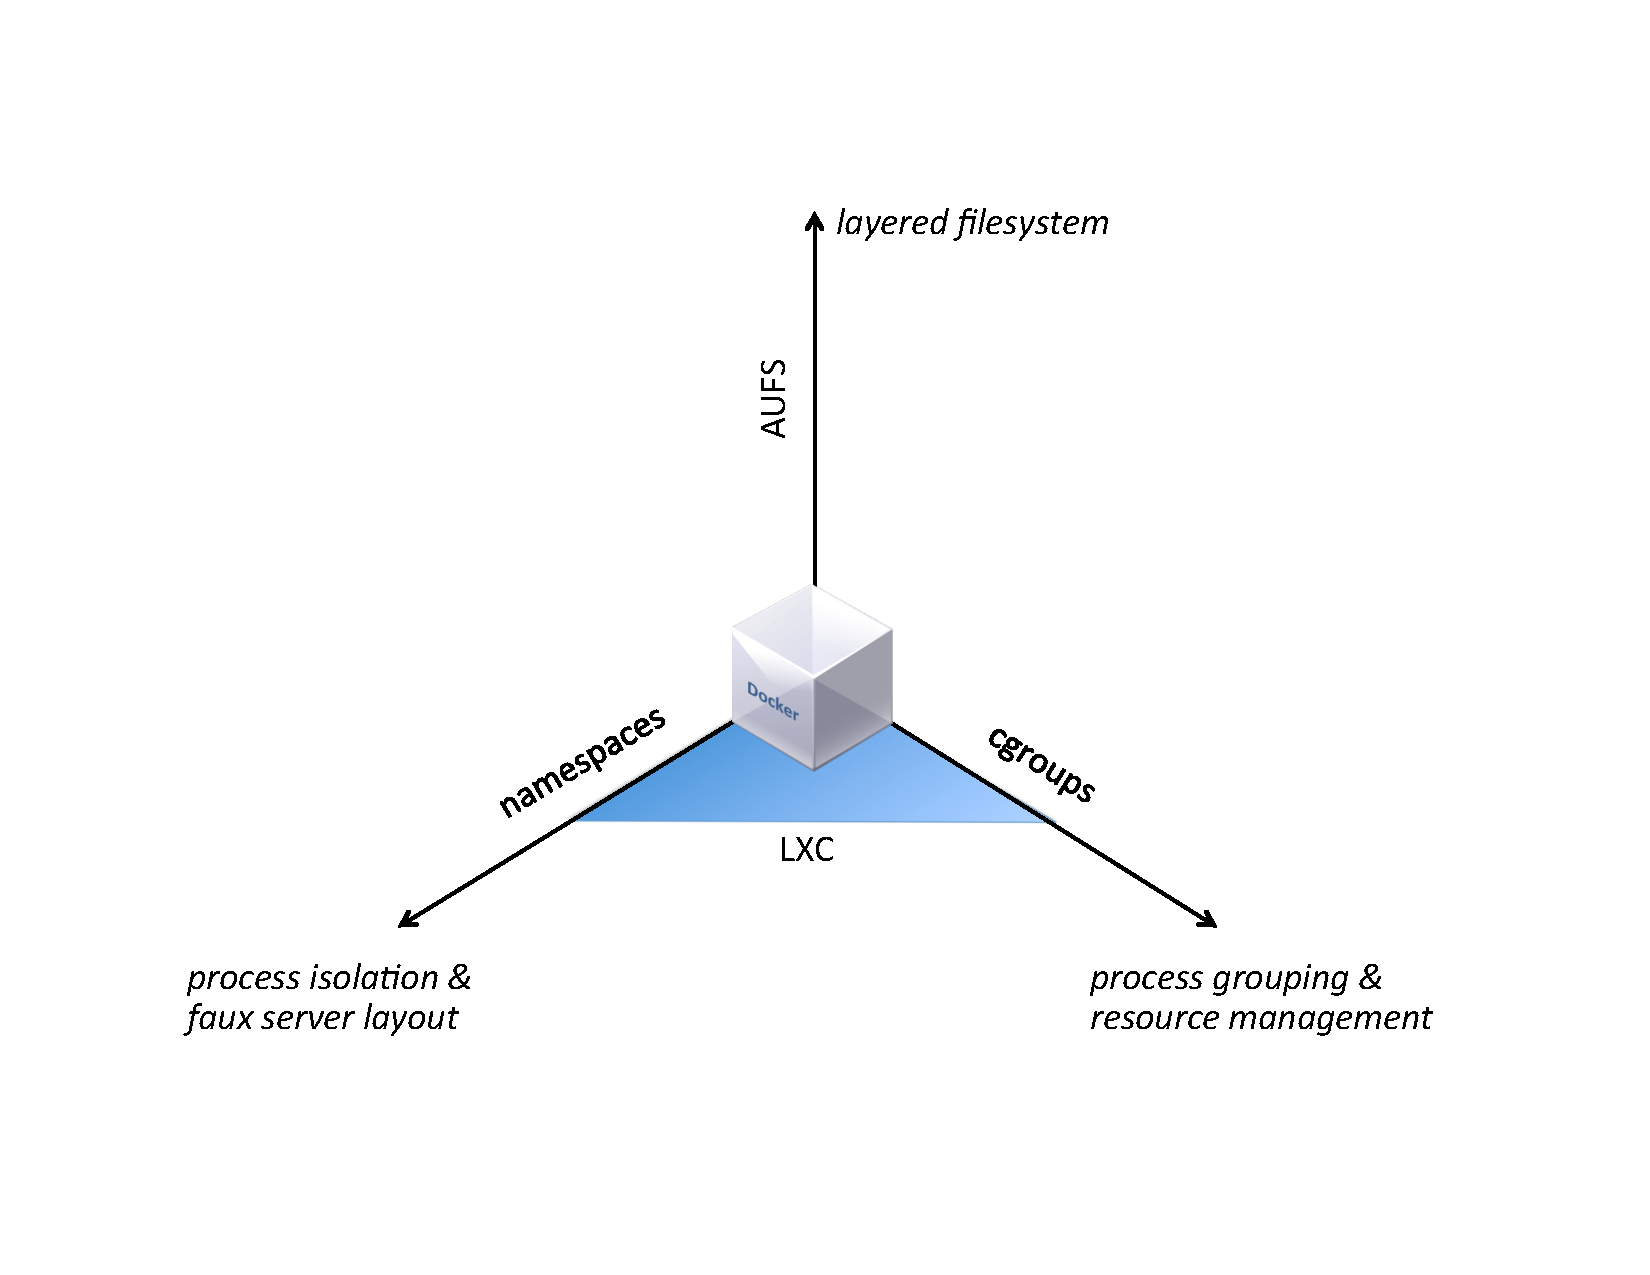
\includegraphics[width=1.0\textwidth]{docker.pdf}
    \caption{A graphic outlining the three fundamental components that make up the Docker framework. Namespace and cgroup support are provided by the LXC (LinuX Container) kernel extensions, and filesystem layering is provided by AUFS.}
\end{figure}

\subsubsection{AUFS}
AUFS, Another Union FileSystem, is the primary means through which Docker achieves both storage savings and faster deployments of containers. Each image inherits from a sequence of other images, up to the base image, and represents the set or sequence of changes on the filesystem. This layering of filesystems and images accomplishes two main benefits. First, it allows for a high degree of storage savings. If two containers are running the same OS and share some libraries and dependencies, the majority of their filesystems will only be represented once on disk and are not duplicated. Second, when downloading and deploying a container, if a host already has previous layers of the filesystem on which a given container depends, it need only download the incremental changes.

\subsubsection{namespaces}
Namespaces are the mechanism by which each Docker container is isolated from the host and other containers. There are many different namespaces that LXC supports, but probably the two most significant ones are the \texttt{pid} and \texttt{net} namespaces. The \texttt{pid} namespace is responsible for giving each container its own isolated environment for processes. A given container can only see and send signals to the processes that are running within the same container. In addition, the \texttt{net} namespace allows different containers to have what appears to be distinct network interfaces, thereby permitting two containers to simultaneously bind to the same port, for example \cite{lxc}.


\subsubsection{cgroups}
Cgroups, or control groups, are a feature on the Linux kernel that provides resource limiting, in the form of memory or disk limits, as well as prioritization of CPU and disk throughput. These features are comparable to those offered by a virtual machine hypervisor to allocate a given amount of memory and CPU, network, and disk priority to a virtual machine.

\subsection{Docker Registry}

Docker provides a public registry to which developers can push their custom Docker images and share their creations with others \cite{dockerregistry}. It has support for creating private images, but requires the user to pay to have more than one privately hosted image.

Docker also has open sourced the Docker Registry \cite{dockerregistry-github} to allow for privately hosted registries. For enterprises, this is a superior solution that allows for easy deployment and configuration of Docker containers across a wide area datacenter.


\section{VMs vs Docker}
\label{sec:vmvsdocker}
While it remains to be seen whether Docker poses an immediate threat to the virtual machine landscape, it is evident that virtual machines and containers are distinct products that aren't necessarily direct competitors. Each caters to a slightly different audience.

Since Docker shares the kernel with the host, it only supports Linux-based containers and immediately discards support for legacy enterprise software that might need a Windows environment to run.

Central to the distinction between container and virtual machine is the tradeoff between density and isolation. Virtual machines offer the strongest form of isolation, comparable to that offered by physically separated hosts. Containers, on the other hand, share the kernel with the host, and therefore provide a much larger attack surface through which an attacker might be able to compromise another container on the same host. 

By giving up isolation, unlike virtual machines which incur a performance overhead, containers achieve near native performance as compared to running directly on the host itself \cite{performance}. Furthermore, the density of containers on a given host can be much higher than that of VMs. 

\begin{figure}[h]
\centering
\subfigure[Docker Container]{%
  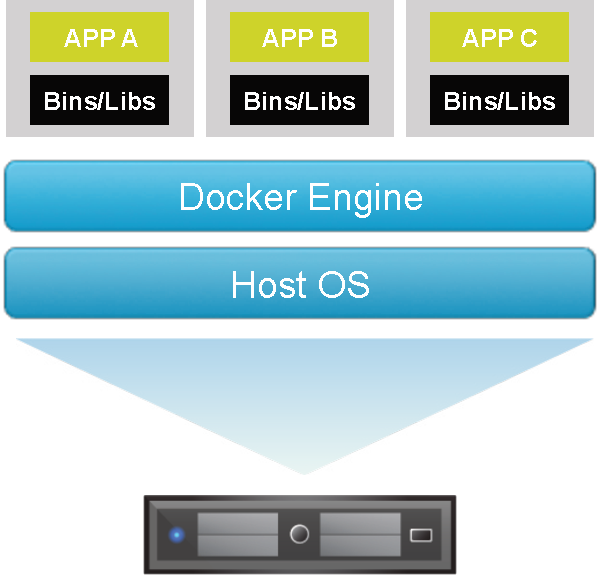
\includegraphics[width=.4\linewidth]{docker_h.pdf}
  \label{fig:sub1}}
\quad
\quad
\subfigure[Virtual Machine]{%
  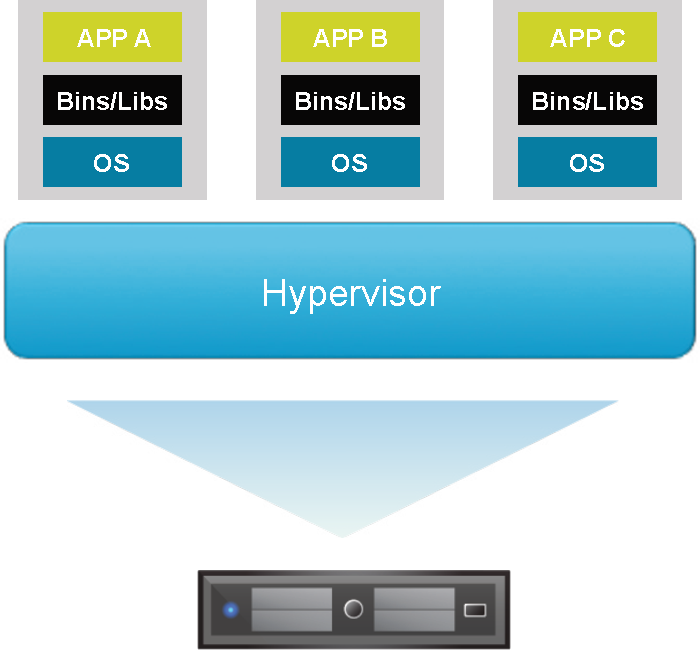
\includegraphics[width=.4\linewidth]{vm_h.pdf}
  \label{fig:sub2}}
\caption{A comparison of the components and isolation of virtual machines as compared to Docker containers. Each container consists of only an application and its dependencies and shares the underlying kernel with the host OS.}
\label{fig:test}
\end{figure}

Since Docker can run directly inside of a virtual machine, but not vice versa, there are interesting ways in which Docker and VMware might be able to work together in the future to offer a streamlined experience that captures the benefits of each. Multiple, trusted, containers running in the same VM, for example, could provide stronger isolation while still achieving the portability and deployment benefits that Docker containers provide.

Another distinct advantage of VMs is there ability to perform live migrations from one host to another. VMware dubs this process vMotion\cite{vmotion}. Docker containers, unless running in a VM (and migrated with vMotion), cannot be live migrated to another host and instead must be shut down, moved, and started back up. CRIU\cite{CRIU} is a project under heavy active active development that attempts to bring this live migration to the container ecosystem by implementing checkpoint/restore functionality for Linux in userspace.


\section{Previous Work}
\label{sec:prevwork}
The existing work in this field is fairly limited, and to the extent of our research there is no existing tool that attempts to automate the conversion from VM to container. Everything must be done manually.


\subsection{Filesystem}

Included with Docker is the import tool that has the following documentation:\\

\texttt{Usage: docker import URL|- [REPOSITORY[:TAG]]}

\texttt{Create an empty filesystem image and import the contents of the tarball (.tar, .tar.gz, .tgz, .bzip, .tar.xz, .txz) into it, then optionally tag it.} \\

Theoretically, this tool would permit us to create a tarball out of a full-fledged virtual machine and import it directly into Docker. However, doing so would completely abandon the notion of layering different filesystems together to construct an image, and the final Docker image would take up the same space as the original virtual machine. Furthermore, if multiple virtual machines were converted in this manner, even if they had the same underlying OS and distribution, their layers wouldn't share any of the same lineage. Thus, two docker images would take up the same amount of space as the original two VMs. 

As a result, Docker recommends that this tool be used only to create base images. In the Docker framework, base images are those images that do not have a parent and instead fully represent an entire OS on their own. Base images are used as starting points from which all other projects can inherit \cite{baseimage}. Base images should be made as small as possible and intuitively should only contain the necessary files to provide a fully-functioning OS. Packages can subsequently be installed on top of the base image depending on the desired function of the container. 

\subsection{Docker2VM}
Unlike the task of converting VMs to Docker, the converse is extremely straightforward. Since Docker can be run within a VM, one can simply run the same Docker container within a VM to obtain a Docker image that has been ``converted" to a VM.s

\section{\projectname}
\label{sec:project}
To this effect, I propose a set of scripts that aids in the conversion from virtual machine to corresponding container or set of containers. Exploiting the benefits of filesystem layering, \projectname\ would reap the benefits of reduced container footprint relative to VMs, as well as achieve the performance gains that containers offer.

\subsection{Filesystem Layering}
A significant component of this endeavor comprises the optimal decomposition of a virtual machine into a set of configuration files and an associated Dockerfile, which together can be used to build a Docker image. Docker's filesystem layering allows multiple images that inherit from the same parent image to share many of the same files, therefore drastically cutting down on the total space needed for many copies or minor derivations of the same base image. In addition to space savings, the corresponding Docker images take up a fraction of the space of a VM and can therefore be downloaded and shared in a much more convenient manner.


\subsection{Dockerfile}
A Dockerfile is a set of instructions that Docker uses to build a new image, given a parent image and a set of commands to execute within the intermediate containers. In addition to running commands, Dockerfiles have the ability to add auxiliary files stored in the same directory as the Dockerfile and insert them into the container's filesystem for subsequent access.

\subsection{Reversible Transformations}
Starting from the original VM, \projectname\ will apply a set of transformations in order to reduce the corresponding size of the set of build files used to generate the Docker image. Only such transformations that can be directly undone (in reverse order) in the Docker build process will be applied. The verification step will ensure that the built image's filesystem is byte for byte equivalent to the original VM filesystem. We will focus on two such reversible transformations: diff and package uninstallation and reinstallation.

\subsubsection{Diff}
The most straightforward way of exploiting layering in Docker is by means of simple Docker image inheritance. Built into the engine is a method by which each image can be told to start from an existing image, identified by a repository and tag name. This could either be a base image corresponding to a specific release of an operating system, or it could be a more complex image, which itself inherits from another image. 

We make use of this layering by automatically detecting the distribution and release of the corresponding VM. As long as the VM is running a release of Linux with a kernel version that exceeds 3.8, it should be supported by \projectname. The distribution and release can be found in \texttt{/etc/*-release} and roughly correspond to the repository and tag name, respectively. Once obtained, we check for the existence of the corresponding base image on the Docker Registry. For now, we are using the publicly available registry but intend to transition to a private registry. A private registry would allow any such base images that are not available on the public registry, like RedHat because of licensing reasons, to be generated on the fly with a tool like \texttt{debootstrap}\cite{debootstrap} and then pushed to the registry.

Once detected, we export the filesystem of the corresponding base image and make use of \texttt{rsync} to generate a diff that represents all of the changes and additions that have been applied from the base image to get to the given VM. We then run another round of \texttt{rsync} in reverse to obtain the set of changes and deletions that have been applied. Cross-referencing these lists, we extract just the deletions and convert them to a list of the filepaths of the deleted files. We create a tarball of all of the changes and additions. Starting from the base image, expanding the tarball and then iterating through the list and deleting each file will yield the filesystem of the original VM. These build instructions are provided in the Dockerfile. 

By making use of a diff, we reduce the size of the VM to the size of the tarball representing the diff and automatically make use of Docker's built in filesystem layering capabilities. For an outline of space savings associated with this technique, see section~\ref{sec:results}.

\subsubsection{Package management}
To further reduce the size of the given diff and maximize the amount of layering, \projectname\ will automatically detect the packages that are installed on the base image of the OS, as compared to those on the VM. Before calculating the filesystem diff, we construct a diff of packages that are installed. While each OS's package management tool differs in commands and syntax, on a high level the process is largely similar regardless of underlying OS. Presumably, the diff will consist of mostly packages that are installed on the VM and not the base image, but it is possible others will exist on the base image but not the VM. We make a clone of the VM's filesystem (so as not to modify it in any way), and then we uninstall all packages on the VM but not the base image and install packages on the base image but not the VM. It is essential to preserve any configuration files that have been customized and will not be restored by the corresponding install process.

The goal of this technique is to further coerce the VM filesystem to be as similar to the base image as possible before calculating the diff, thereby reducing its size. During the build process, after applying the diff we can reinstall any packages that had been removed and vice versa, thereby obtaining the original VM filesystem.

TODO: use a directed graph to calculate dependencies and reduce the number of packages listed.

\begin{figure}[h]
\centering
    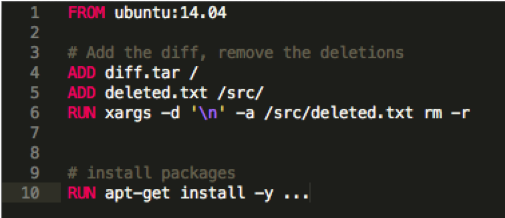
\includegraphics[width=0.6\textwidth]{dockerfile.png}
    \caption{An example Dockerfile generated by \projectname\ which exploits Docker's built in layering. Undoing the changes applied to the VM in the reverse order, we obtain the original VM's filesystem. First, we inherit from the base image of the corresponding Linux distribution and release. Then, we add the tarball of changes and deletions, which Docker automatically unpacks. We then add the list of deleted files and execute a command to delete all of the files listed. Finally, we install any packages detected on the VM but not the base image, using the provided package management tool.}
\end{figure}


\subsection{Additional Space-Reducing Techniques}
Certain files in the VM are either unnecessary, or can be regenerated on the fly. Since Docker containers share their kernel with the host operating system, they disregard any kernel modules that are provided in the container. Thus, we can safely remove these associated files from the diff in order to save space. Furthermore, the package repository cache takes up a fair amount of space, and is used only for performance reasons. This can be safely purged from the filesystem without affecting correctness. For Ubuntu, these files are located at \texttt{/var/cache/apt/pkgcache.bin} and \texttt{/var/cache/apt/srcpkgcache.bin} and can potentially take up about 100 MB.

\subsection{Verification}
With all of these transformations in place, it is essential to verify that the Docker image that is built is identical to the original VM in terms of its filesystem. Theoretically, since we are applying a sequence of transformations on the VM, and then applying the reverse sequence of inverse transformations during the build process, the resulting Docker image should be identical. Nonetheless, we implement this optional method of image verification to ensure correctness. Image inheritance and diff creation and patching is relatively straightforward and well-tested. On the other hand, package uninstallation and installation may not always be exact inverse operations, which might affect correctness of the Docker container. Although package management provides an opportune strategy to cut down on the size of the image diff, it is potentially risky and should be used with caution.

\subsection{Container Configuration}
In addition to converting the filesystem to one that may better exploit layering, another big component of \projectname\ is its ability to automatically configure the resulting containers in a manner similar to that of the original VM.

Unlike VMs which start up an entire operating system, Docker containers are started by running a specific command in the shell. This command can correspond to running the \texttt{init.d} startup script which will in turn start up and monitor as many other processes as needed. Alternatively, each container may also correspond to a single process. In this paradigm, the command that runs the container corresponds to the command to start up the given process, and each VM may potentially map to multiple containers. With multiple containers in place, there becomes a need for multi-container orchestration, which enables the linking of multiple containers together so that they may communicate and potentially share volumes without having direct knowledge of the other's IP address until runtime. 

Although Docker doesn't directly support this degree of orchestration, there are existing frameworks in the field that include fig\cite{fig}, kubernetes\cite{kubernetes}, and fleet\cite{fleet}. They each function by parsing a given configuration or set of configuration files on startup. We envision \projectname\ providing optional support for all of these frameworks, with a command-line option being able to specify which should be used during conversion.

When running directly on the VM host, \projectname\ can automatically detect the currently running processes that were kickstarted at startup, as well as the commands used to start them using \texttt{ps}. Furthermore, we use \texttt{netstat} to determine which processes are bound to certain ports, to be sure to expose the corresponding ports through Docker.

Finally, in terms of resource allocation, we can parse the VMX file provided with a given virtual machine to determine its specific resource allocation. In the case where we are mapping 1 VM to 1 container, it is straightforward to provide the container with the same resource restrictions and allocations as its corresponding VM. For more complex mapping schemes, some sort of user intervention may be required in the form of a prompt to generate reasonable resource restrictions for each container.

\subsection{Deployment}
As of this writing, the prototype of \projectname\ is a Python command-line program that is called by passing in the path to the root of the Virtual Machine filesystem. In effect, this is done by running the conversion script in an additional VM, which has mounted the VMDK of the VM to be converted. Since VMware software can itself mount VM disks (VMDK), this was the most straightforward method of obtaining access to the root filesystem of the VM. 

However, this method of conversion leaves much to be desired, as it requires each target VM to be manually mounted through the VMware user interface. The current prototype is therefore feasible for testing, but would quickly become unwieldy as the number of VMs approached hundreds or thousands. Furthermore, for base images that aren't available on the public Docker registry, \texttt{debootstrap} is needed and must be run directly on the given host.

As a longterm goal, \projectname\ should be able to be run on an entire virtual datacenter, and the virtual resources of a given VM should be able to be used in a distributed manner. In this way, the vSphere API could be used to streamline the simultaneous conversion of many VMs to Docker images, without requiring any more additional compute resources than those already available and in use.

Similar to how existing tools are used to convert a physical host to VM, a self-contained executable could be downloaded and executed on a given host that would run the migration process from VM to container, or determine that the VM is not supported. Currently, the migration tool itself depends on the \texttt{rsync} utility, Python 2.7, the Python Docker client API, and an additional Python library called networkx. Additionally, the Docker command-line client is needed for importing base images from a tarball, since the Python library is largely inefficient.

Such an executable would need to install the required dependencies in an isolated part of the filesystem, then convert the VM to Docker using the existing tool while ignoring the dependencies needed to use the tool, and then push this new Docker image to a privately hosted registry for subsequent access and deployment.

\section{Preliminary Results}
\label{sec:results}
Thus far, we have focused on the filesystem aspect of the virtual machine conversion process. The results show a promising start to our goal of reducing the size of the resulting Docker containers by exploiting layering. For our data, we ran a prototype of the conversion script on six major releases of the Ubuntu distribution between 10.04 and the current 14.04 release. The scripts focus on just two of the aforementioned strategies for cutting down on the VM sizes:

\begin{enumerate}
\item Match up the VM with an existing base image and create a diff of the two
\item Detect existing installed packages (differs by distribution) and generate commands to reinstall them, rather than included these packages in the diff.
\end{enumerate}

We present the results of the first strategy, and then the two combined strategies, in the table and graphs below:

\subsection{Diff-Based Layering}
We match up each VM with its corresponding base image and then perform a diff using \texttt{rsync} to define the VM in terms of a set of additions, deletions, and changes applied to the base image. Table~\ref{table:diff} shows the space savings obtained by this process. Although the absolute reduction in space between the VM and the diff is relatively small, of interest is the amount of space saved relative to the base image. Since the diff is obtained relative to the base image, the maximal possible savings occurs if the VM represents only additions on the base image and the size reduction would be exactly equal to the size of the base image. We observe that the VMs are able to save between 35 and 72 \% of the size of the corresponding base image by taking advantage of layering and diffs. This space savings would manifest itself not only in a reduction of size of the container. In addition, assuming many containers inherit from the same image, it would also result in a reduction of time it takes for the container to be downloaded from a repository, a nontrivial performance benefit.

\begin{table}[h]
\centering
    \begin{tabular}{| c | c | c | c | c | c | c |}
    \hline
& \multicolumn{6}{|c|}{\bfseries Ubuntu Release} \\ \hline
    \bfseries Size (MB) & \itshape 10.04 & \itshape 12.04 & \itshape 12.10 & \itshape 13.04 & \itshape 13.10 & \itshape 14.04 \\ \hline
    \bfseries VM & 713 &  895 & 714 & 723 & 1006 & 1143\\ \hline
    \bfseries Base Image & 174 & 79 & 144 & 141 & 155 & 171  \\ \hline
    \bfseries Diff & 652 & 846 & 638 & 650 & 932 & 1020\\ \hline \hline
    \bfseries \% Saved & 35.1 & 62.0 & 52.8 & 51.8 & 47.7 & 71.9\\
    \hline
    \end{tabular}
\caption{The table above shows the space savings, compared to the original VM size, of converting to a Docker image that layers on top of the base image. The last row outlines the percentage of space saved, relative to the base image. 100\% would denote that the diff is exactly equal to the VM minus the base image.}
\label{table:diff}
\end{table}


Based on these results, we see that matching up a VM with a corresponding base image and calculating a diff alone begins to reap the benefits of Docker's layered container filesystem. In addition to this approach, the detection of installed packages available through the \texttt{apt} repository has further ability to drastically cut down on the weight and size of these VM-based containers.

\subsection{Package Management}

Another method of exploiting layering we used is based on the detection of the packages currently installed using the existing package manager. These packages, instead of being directly represented in the tarball of the diff, could be listed as a set of packages to be installed after the diff has been applied to the base image. As long as each package's uninstall and reinstall process are inverses and package configuration files are left as-is, the transformation would leave the resulting Docker container identical to the original.

Since most of the differences between the base image and the VM come in the form of packages, this package management strategy had the most significant impact on the resulting size of the diff. Of course, since the packages still need to be reinstalled on the container, the resulting container size is exactly the same. However, the package used to build this image is substantially smaller, which means the deployment time and portability of the package is improved.

The following table shows the reduction in diff sizes for various releases of Ubuntu, as obtained by applying the technique of package management and subsequent installation.

\begin{table}[h]
\centering
    \begin{tabular}{| c | c | c | c | c | c | c |}
    \hline
& \multicolumn{6}{|c|}{\bfseries Ubuntu Release} \\ \hline
    \bfseries Size of Diff (MB) & \itshape 10.04 & \itshape 12.04 & \itshape 12.10 & \itshape 13.04 & \itshape 13.10 & \itshape 14.04 \\ \hline
    \bfseries Before & 652 & 846 & 638 & 650 & 932 & 1020\\ \hline
    \bfseries After & 349 & 374 & 208 & 194 & 424 & 540  \\ \hline \hline
    \bfseries \% Reduction & 46.5 & 55.8 & 67.4 & 70.2 & 54.5 & 47.1\\
    \hline
    \end{tabular}
\caption{The table above shows the space savings, compared to the original diff size, of using a method of package management to further reduce the size of the diffs. The results reduced the size of the diff by between 46 and 70\%  and helped maximize portability of the resulting Docker build instructions.}
\label{table:diff}
\end{table}

Further experimentation will be done with various releases of other Linux distributions such as CentOS, RedHat, Gentoo, BusyBox, Debian, and Fedora.



\section{Evaluation}
\label{sec:evaluation}
In addition to implementation, the results of the thesis can be evaluated in a number of objective and straightforward ways: 
\begin{itemize}
\item Compile filesystem data for image sizes and diff sizes for other Linux distributions, such as CentOS, RedHat, and Gentoo
\item Attempt to quantify the time it takes to convert a VM to Docker container. This would largely vary depending on the VM, but mean and median statistics can be compiled.
\item Describe and quantify the tradeoff between decreasing image size and increasing build time of Docker container
\item Determine the efficiency of converting an entire virtual datacenter to Docker, capturing before and after space usage as well as performance metrics for standard tasks.
\item Establish a measure for the ability to convert VMs to containers without any user intervention, including what kinds of VMs can be seamlessly converted.
\end{itemize}

\section{Further Research}
\label{sec:futureresearch}
If time permits, we would like to explore supporting the conversion of vApp to a set of containers. vApps are a logical set of Virtual Machines that work together to support a specific applications goals. This would likely map to a set of containers, where each container corresponds to a a given virtual machine. Just as the VMs are linked together through perhaps shared volumes and network communication, the containers' could be orchestrated to function in an analogous manner.


\begin{thebibliography}{99}

\bibitem{lxc}
``PaaS under the hood, episode 1: kernel namespaces," November 28, 2012. [Online]. Available: \href{http://blog.dotcloud.com/under-the-hood-Linux-kernels-on-dotcloud-part}{http://blog.dotcloud.com/under-the-hood-Linux-kernels-on-dotcloud-part}

\bibitem{dockerregistry}
``Docker Hub Registry," [Online]. Available: \href{https://registry.hub.docker.com}{https://registry.hub.docker.com}

\bibitem{dockerregistry-github}
``Docker Registry," 2014. [Online]. Available: \href{https://github.com/docker/docker-registry}{https://github.com/docker/docker-registry}

\bibitem{performance}
M. G. Xavier, M. V. Neves, F. D. Rossi, T. C. Ferreto, T. Lange, and C. A. F. De Rose, ``Performance Evaluation of Container-based Virtualization for High Performance Computing Environments," 2013. [Online]. Available: \href{http://marceloneves.org/papers/pdp2013-containers.pdf}{http://marceloneves.org/papers/pdp2013-containers.pdf}

\bibitem{vmotion}
``VMware vMotion: Virtual Machine Live Migration," [Online]. Available: \href{http://www.vmware.com/products/vsphere/features/vmotion}{http://www.vmware.com/products/vsphere/features/vmotion}

\bibitem{CRIU}
``CRIU," 2014. [Online]. Available: \href{http://criu.org/}{http://criu.org/}

\bibitem{baseimage}
``Creating a Base Image," 2014. [Online]. Available: \href{https://docs.docker.com/articles/baseimages/}{https://docs.docker.com/articles/baseimages/}

\bibitem{debootstrap}
``Debootstrap," [Online]. Available: \href{https://wiki.debian.org/Debootstrap}{https://wiki.debian.org/Debootstrap}

\bibitem{fig}
``Fig | Fast, isolated development environments using Docker," 2014. [Online]. Available: \href{http://www.fig.sh}{http://www.fig.sh}

\bibitem{kubernetes}
``Kubernetes," 2014. [Online]. Available: \href{https://github.com/GoogleCloudPlatform/kubernetes}{https://github.com/GoogleCloudPlatform/kubernetes}

\bibitem{fleet}
``Launching Containers with fleet," 2014. [Online]. Available: \href{http://coreos.com/docs/launching-containers/launching/launching-containers-fleet/}{http://coreos.com/docs/launching-containers/launching/launching-containers-fleet/}



\end{thebibliography}

\end{document}
